\documentclass[11pt, a4paper,nomath,nopackage]{siltex-report}
\usepackage{amsmath}
\usepackage[nomath]{siltex}
\usepackage[language=nl]{bauwatchtitle}
\usepackage{graphics}
\usepackage{pdflscape}
\usepackage{multirow}
\usepackage{tabulary}
\usepackage{float}
\usepackage{listings}
\usepackage[acronym]{glossaries}
\usepackage[style=ieee]{biblatex}
%\usepackage[hidelinks]{hyperref}

\usepackage{zref-savepos}

\addbibresource{refs.bib}

\definecolor{black}{rgb}{0,0,0}

\graphicspath{ {./img/} }

\newcommand\YAMLcolonstyle{\color{red}\mdseries}
\newcommand\YAMLkeystyle{\color{black}\bfseries}
\newcommand\YAMLvaluestyle{\color{blue}\mdseries}

\makeatletter

% here is a macro expanding to the name of the language
% (handy if you decide to change it further down the road)
\newcommand\language@yaml{yaml}

\expandafter\expandafter\expandafter\lstdefinelanguage
\expandafter{\language@yaml}
{
  keywords={true,false,null,y,n},
  keywordstyle=\color{darkgray}\bfseries,
  basicstyle=\YAMLkeystyle,                                 % assuming a key comes first
  sensitive=false,
  comment=[l]{\#},
  morecomment=[s]{/*}{*/},
  commentstyle=\color{purple}\ttfamily,
  stringstyle=\YAMLvaluestyle\ttfamily,
  moredelim=[l][\color{orange}]{\&},
  moredelim=[l][\color{magenta}]{*},
  moredelim=**[il][\YAMLcolonstyle{:}\YAMLvaluestyle]{:},   % switch to value style at :
  morestring=[b]',
  morestring=[b]",
  literate =    {---}{{\ProcessThreeDashes}}3
                {>}{{\textcolor{red}\textgreater}}1     
                {|}{{\textcolor{red}\textbar}}1 
                {\ -\ }{{\mdseries\ -\ }}3,
}

% switch to key style at EOL
\lst@AddToHook{EveryLine}{\ifx\lst@language\language@yaml\YAMLkeystyle\fi}
\makeatother

\newcommand\ProcessThreeDashes{\llap{\color{cyan}\mdseries-{-}-}}


\newcounter{NoTableEntry}
\renewcommand*{\theNoTableEntry}{NTE-\the\value{NoTableEntry}}

\newcommand*{\notableentry}{%
  \multicolumn{1}{@{}c@{}|}{%
    \stepcounter{NoTableEntry}%
    \vadjust pre{\zsavepos{\theNoTableEntry t}}% top
    \vadjust{\zsavepos{\theNoTableEntry b}}% bottom
    \zsavepos{\theNoTableEntry l}% left
    \hspace{0pt plus 1filll}%
    \zsavepos{\theNoTableEntry r}% right
    \tikz[overlay]{%
      \draw[red]
        let
          \n{llx}={\zposx{\theNoTableEntry l}sp-\zposx{\theNoTableEntry r}sp},
          \n{urx}={0},
          \n{lly}={\zposy{\theNoTableEntry b}sp-\zposy{\theNoTableEntry r}sp},
          \n{ury}={\zposy{\theNoTableEntry t}sp-\zposy{\theNoTableEntry r}sp}
        in
        (\n{llx}, \n{lly}) -- (\n{urx}, \n{ury})
        (\n{llx}, \n{ury}) -- (\n{urx}, \n{lly})
      ;
    }% 
  }%
}

%%%%%%%%%%%%% Content below %%%%%%%%%%%%%

\title{Camera Provisioning}
\author{Thymo van Beers}
\date{February 2022}

\begin{document}

\begin{titlepage} 
\maketitle
\vspace*{\fill}
Status: Draft
Version: 0.1
Student number: 452434
Degree: Software Engineering
Saxion University of Applied Sciences
Bachelor Thesis
\thispagestyle{empty}
\end{titlepage}
\newpage


\section{Contact information}
\begin{center}
\begin{tabular}{ | m{8em} | m{8em} | m{8em} | m{11.1em} | }
\hline
\textbf{Name} & \textbf{Organization} & \textbf{Function} & \textbf{E-mail}
\\ \hline
Thymo van Beers & BauWatch Technology Group & Graduate student & thymovanbeers@gmail.com
\\ \hline
Wouter Horlings & BauWatch Technology Group & Company mentor & whorlings@bouwatch.nl
\\ \hline
Peter Ebben & Saxion & Saxion mentor & p.w.g.ebben@saxion.nl
\\ \hline
Willem Prakken & Saxion & Graduation coordinator & w.prakken@saxion.nl
\\ \hline
\end{tabular}
\end{center}
\newpage
\section{Acknowledgements}
TBD
\newpage
%TODO Disable pagenumbering
\section{Summary}
This will be written at the end, max 1 page.
\newpage

\thispagestyle{empty}
\tableofcontents
\thispagestyle{empty}
\newpage

\section{Introduction}
BauWatch is a security system supplier that develops and operates temporary video surveillance and access control systems for use at construction sites and other remote locations.
One of their most popular products are the video masts (called a "BauWatch"), a portable, self-contained, metal enclosure including an internal
power source, network connectivity and a telescopic mast with cameras, green floodlights and other peripherals. A BauWatch can be lifted by a forklift and
easily transported to the next location. Research \& Development for these products is done by BauWatch Technology Group (BTG) located in Enschede.

\section{Company history}
FIGO was created in 2007 as a product line of the Twente Institute for Wireless and Mobile Communications (TI-WMC). The name FIGO comes from the Italian word meaning:
fig, cool, tasteful, sexy.
They used to focus on network equipment but now also handle the cameras in the video masts
In 2018 they were acquired by BauWatch to form their R\&D department under the name BauWatch Technology Group.
BauWatch has a backend team under which I do my research.

BauWatch Technology Group has its roots at the Ericsson research facility that was housed in Enschede until 2003. During the 90s and early 2000s Ericsson was doing
research on DECT, Bluetooth, 3G and WiFi. After Ericsson closed their Enschede facility the Twente Institute for Wireless and Mobile Communications (TI-WMC) was created as a technology R\&D spin-off specialized in wireless mobile communications systems. The result of various networking related projects were combined in its product line FIGO that combines Wi-Fi-based multi-radio meshing with cellular and Ethernet connectivity for public safety applications. \cite{ti_wmc}

In 2011 FIGO was split-off to be a sister organization to TI-WMC focusing on the sales and further development of the FIGO product. After TI-WMC defaulted in 2014, FIGO
continued alone at a new location where it still is today. The years after the split, FIGO did various contracted projects like Sensor City Assen, Bad Boys Buster with
Luminoxx, and BauWatch. After various projects with BauWatch, they acquired FIGO in 2018 to become its dedicated R\&D department after which it no longer focused solely on networking equipment but also doing more work with the cameras and Network Video Recorders (NVR) used by BauWatch.


\section{Scope}
% The project has commence on 15-11-2021 and will be completed by 22-04-2022. The scope of the project will be limited to the configuration of cameras through their APIs only. No modifications 
% will be done to the firmware of cameras and no special consideration is given to BauWatch' network architecture other than the cameras being reachable on a unique IP-address. Furthermore the focus of the prototype will be with the manufacture API instead of ONVIF. ONVIF will only be used
% in the specific case a part of the manufacturer API is found not to be working properly or if implementing a call to the API would cause an unacceptable delay.
% If during the project it is determined that the implementation of the prototype will finish early, an addition can be made to add the ability for equipment other than cameras (speakers,
% lights, etc.) to be configured.
% The design for the prototype will not add any specifics regarding other equipment but will be designed in such a way that this addition can be made without much effort if required.

% The first camera that will be investigated is a Hikvision DS-2DE4225IW-DE. BauWatch expressed that these cameras will be more actively used in the future and that it would be nice to have a working prototype using this camera model. The second camera that will be investigated is a VCA IPX3802SV because it
% provides a different API from the Hikvision and is actively in use within BauWatch.

The project commenced on November 15th 2021 and ended on April 22nd 2022. The scope of the project was limited to the configuration of cameras through their own APIs only and
without making any firmware modifications. Since only a proof of concept was to be made, no special consideration to BauWatch' network architecture was given although it became
evident that this wouldn't cause any obstacles either since all cameras can be reached on a unique IP-address.
%During the definition phase of the project a thesis on implementing
%an ONVIF plugin was found. To prevent overlap the project was reformulated so that ONVIF would not be required, the prototype could however support an interface to ONVIF in the
%future if such an interface is deemed necessary.

Two cameras were used for the project. Namely, a Hikvision DS-2DE4225IW-DE and a VCA IPX3802SV. These were selected based on the different ways the API works
and their current or expected increased future usage in the video masts.
\newpage
% Bauwatch heeft verspreid door EU meer dan 10k cameras in het veld. Momenteel is er geen toereikende methode om al deze cameras te beheren.
% Zonder een toereikende beheeroplossing is het niet mogelijk om een goed overzicht te houden van welke camera over welke instellingen beschikt.
% De huidige werkwijze is om de camera's vanuit de fabriek eenmaal met de juiste instellingen te configureren.
% Na deze eerste configuratie is het niet toegestaan om deze instellingen aan te passen.

% Desondanks zijn er situaties waar een alternatieve configuratie gewenst is omdat het de kwaliteit van de bewaking verhoogt. In sommige
% situaties wordt deze alternatieve configuratie wel toegepast ookal is de werkwijze om dit niet te doen.
% Wanneer een camera naar een andere locatie wordt verplaatst is er geen manier om in te zien of de configuratie nog klopt.
% Hierdoor kan een camera met een specifieke configuratie op een andere locatie terecht komen.
% Het gevolg hiervan is dat de camer niet meer naar verwachting werkt.

%Peter:
% How does it work now?
% 



\section{What parameters are of interest to BauWatch?}
Cameras include a lot of settings that could be relevant to BauWatch.
It's good to know what parameters should be implemented into the prototype and what parameters are still relevant, but don't directly add value to the prototype as their implementation would be very similar to others.
In order to determine the parameters that are relevant to BauWatch an interview was conducted on January 11th 2022 with Alex van der Leij, a product manager responsible for the video masts deployed around Europe.

\section{How would the system architecture of a centralized parameter system be designed and implemented?}
Once it is known how a configuration can be represented this should then be applied to the design of the prototype. This design will then be implemented into a
prototype to demonstrate the concept using a couple of parameters that BauWatch deems relevant.

% While preparations were being made for this project some preliminary library research has been conducted. During this period a previous thesis on creating an ,,ONVIF Plug-in" \cite{tim_k_onvif} was found. This thesis was found to contain a lot of material that would have been produced in the original scope of the project. This caused some
% delays during the definition phase of the project as the scope of the assignment had to be slightly adjusted to prevent doing redundant work. 
% The new project that was defined aims to improve areas where ONVIF does not apply. Cameras do not always implement all components through ONVIF
% or if they do they may not properly follow the specification. These cameras do however have their own API that is known to operate properly.

\chapter{Design}
\label{sec:design}
In this chapter the design for the Camera Provisioning system will be laid out.
The goal of the system is to provide a solution which makes it possible to manage camera configurations.
The system allows the user to orchestrate parameters into different templates which can be assinged to a camera.
The design will contain both functional and technical specifications containing the descriptions of different components, requirements and supplemental diagrams and wireframes.
\section{Requirements}
In table \ref{tab:requirements} the requirements for the system have been defined. Requirements are tracked using an identifier starting with a letter followed by a
number and are listed in the ID column of table \ref{tab:requirements}. If the identifier starts with the letter 'B' or a 'U' they specify a business or user requirement respectively. If the identifier starts with a 'F' or 'NF' they specify a functional or non-functional system requirement respectively.
Requirements have been prioritized using the MoSCoW method \cite{noauthor_moscow_nodate}.
\begin{table*}[h]
    \centering
    \begin{tabulary}{\linewidth}{CLL}
        \textbf{ID} & \textbf{Requirement} & \textbf{MoSCoW}
    %%% Business requirements
        \\ \hline %% Check this with NF-7
        B1 & A camera can be configured by the user without detailed knowledge about the model being used & Must
        \\ \hline
        B2 & A camera configuration can be rolled back to any compatible version in history & Must
        \\ \hline
        B3 & The configuration changes must include auditing: show the author and timestamp & Must
        \\ \hline
        B4 & Translated parameters that are scaled to a particular value should be tuneable & Should
        \\ \hline
        B5 & The application has the option to show the user the differences between the config in the camera and the template & Must
    %%% User requirements
        \\ \hline
        U1 & A user can login using a username \& password & Could
        \\ \hline
        U2 & A user can change his credentials through the web interface & Could
        \\ \hline
        U3 & The template used for configuring cameras must include one setting representing a text-field and one setting representing a slider value & Should
        \\ \hline
        U4 & New settings can be added to the application without having to change the templates & Must
        \\ \hline
        U6 & The application must be able to handle one or more settings in a template that are not present in any of its parents & Should
        \\ \hline
        U7 & A user can interface with the system using a webbrowser & Should
        \\ \hline
        U8 & A user can create a new template with a specified parent template & Must
        \\ \hline
        U9 & A user shall be able to trigger the configuration on one or all cameras according to their template & Must
    %%% System requirements
        \\ \hline
        NF-1 & Communication with cameras are authenticated through HTTP Basic or Digest & Must
        \\ \hline
        NF-2 & The code must be compiled crossplatform & Must
        \\ \hline
        NF-3 & The codebase must be covered with linting. & Must
        \\ \hline
        NF-3 & The codebase shall be strongly typed. & Should
        \\ \hline
        NF-3 & All code shall be covered by unit tests & Must
        \\ \hline
        NF-4 & Templates and camera configuration are stored on disk in a human-readable/typeable format & Must
        \\ \hline
        NF-5 & Templates and camera configuration can be loaded from YAML files & Must
        \\ \hline %% TODO check this with Wouter. Not SMART
        NF-6 & The application should be exposed as a RestAPI and documented via OpenAPI & Should
        \\ \hline
        NF-7 & The templates must be camera independent. & Must
    \end{tabulary}
    \caption{Requirements}
    \label{tab:requirements}
\end{table*}

\section{General design}
At the conclusion of this project the prototype is handed over to the back-end team of BauWatch.
Since they will be further developing the prototype into a production ready system the choice was made to implement the system in Go as that programming language is their preferred language for new products fulfilling requirement NF-2.

\section{Templates}
The provisioning server will have a user interface through which a template can be configured.
A template in the context of this system is a collection of lists containing camera configuration options.
Templates can be built up from different layers where each layer can override parameters from the layer above.
This allows the user to define a template that is shared by a large amount of cameras but still provides more fine-tuned control for certain situations.
These cameras would still use all the settings from the parent template but would have a different setting for camera sensitivity.

\section{Datastructure}
Templates are represented in memory as a tree using dynamically allocated nodes that have pointers to one parent and zero or more children.
There is a single template that is considered to be the root node of the tree.
All templates that are added to the system will be a child of this root node.
The choice to represent the collection of templates as a tree is to solve the requirement of parameter inheritance.
Using this datastructure is an efficient method to enumerate the values of a template's parameters at configuration time.
A parameter can be found by traversing each parent node starting from the node representing the current template until a value for a given paramater is found.
The process of finding a paramater is depicted in figure TBD % TODO add figure
The best-case performance for a parameter lookup is O(1) in the case the parameter is already defined in the current template.
The worst-case performance of a lookup is O(n) where n is the number of templates to be traversed from the current node to the root node.
When a new template is instantiated, by creating a new one or loading one from YAML, that template has to be inserted at the correct place inside the tree.
The way this is achieved is to do a breadth-first search (BFS) in the tree where a match is identified using the name of the parent node.
Using BFS to find the parent node is more efficient than a depth-first search (DFS) as a template is more likely to inherit from a more generic template describing e.g. paramaters for a country than a more specific template representing paramaters for a specific building site. % TODO Proof?

\section{Multiple base templates} %TODO: Root template requires more intro?
While this design requires a single root template that all other templates inherit from, the design still allows the creation of multiple trees with independendant parameter sets.
This can be done by not setting any paramaters in the root template such that the templates directly below it don't have any parameters that can be inherited from the root template.
The children of the root template then become the first template to define the template effectively turning into root templates themselves while still being children of the actual root template.

\subsection{Parameters}
%TODO: How are the templates kept in memory. Describe the parameter interface
%TODO: How will stuff look in the main application
TBD Once I figure out how to properly abstract them in Go.
At the moment only integer parameters are supported.

Cameras can contain many different kinds of parameters. To handle these in a generic way some kind of abstraction needs to be done.
Parameters 

\section{Storing to file}
Templates are stored on disk as YAML formatted data. YAML was chosen because it is a plain text format that can be interpreted by humans while still being able to describe all attributes that make up a template. 
Due to the plain text nature this also allows the usage of tools like GNU diff to produce a view of the differences between two templates.
An example of a YAML-formatted template can be found in listing \ref{lst:template}.
The following data is used to describe a template in YAML:
\begin{itemize}
	\item name: The name of the template.
	\item parent: The name of the parent template this template should inherit from.
	\item parameters: A list of all the parameters contained in this template.
	\item type: A name that defines the type of a parameter.
	\item name: (under parameters): The name of the parameter.
	\item attributes: A generic list with data used to construct a paramater of the type in the `type` key.
\end{itemize}
\lstinputlisting[language=yaml,caption={Example template YAML},label={lst:template}]{format.yaml}

\section{Reading from file}
Templates are stored on disk with the name of the parent. When this file is reloaded to instantiate a template the system must be able to discover its
parent by its name. This can be achieved using a breadth-first search of the template tree.
The operation of loading a template and linking these to their parent is described in figure \ref{fig:inserttemplate}.

\begin{figure}[h!]
	\centering
	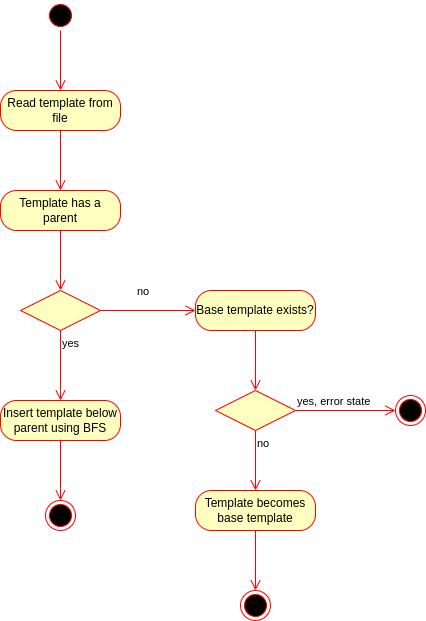
\includegraphics[scale=0.5]{insert_template_acty}
	\caption{Template insert operation}
	\label{fig:inserttemplate}
\end{figure}

\section{Keeping revision history}
In order to fullfill the ability to restore a template to a previous version a revision history is kept.
Templates are stored in a directory with the name of that template.
Inside that directory a template is stored as a file named with the revision number and the file extension (.yml).
This way the latest revision can be found by sorting the files by name in descending order.
When a template is reverted to a previous version the files will be sorted in the same manner and will be deleted until the revision to revert to is reached. An example of how this directory structure would be stored is seen in figure \ref{fig:diskstruct}

Storing templates in this manner has one flaw.
Namely that of sorting by name when more than 10 revisions have been made.
A solution to this problem could be to use leading zeroes to delay the problem or to sort on a different attribute, like file modification time.

One off the shelf solution for versioning files that cannot be ignored is git.
Git is originally intended to keep track of program source files but can also be used for other kinds of files.
The goals of git are speed, data integrity and distritbuted workflows.

Argument: Is git overkill? Why use it or the other suggested solution. Make a choice.

Design:
Each time a template is saved it is saved as a yaml file and committed in git.
A commit only modifies one file at a time.
A template can be reverted to an earlier commit.
Author information is entered at the login screen.
library available that implements porcelain functions.

\begin{figure}[h!]
	\centering
	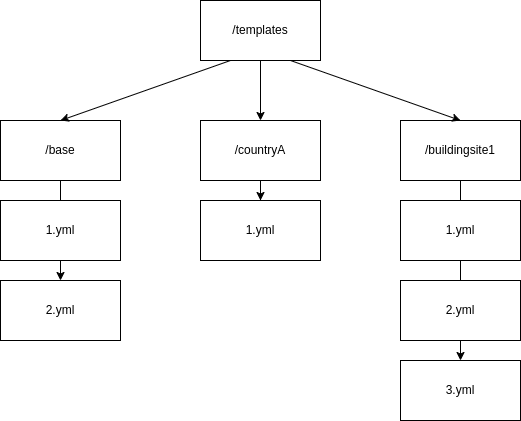
\includegraphics[scale=0.5]{yaml_dir_struct}
	\caption{Directory structure of templates and their revisions}
	\label{fig:diskstruct}
\end{figure}

\subsection{Camera interface}
The camera interface is a system component that sits between the template component and the cameras themselves. The purpose of this component
is to translate the settings from a template into an API call understood by the camera. Each camera can have a different API with potentially different interpretation of parameters. This component will map the parameter from the template to an appropriate value for that camera.
In order for a camera to accept new parameters they require a form of authentication. All cameras being used support both HTTP Basic and HTTP Digest authentication.
To successfully interface with the cameras one or both of these authentication methods must be supported by the camera interface component.

\subsection{Translating generic parameters to camera specific values}
As an example of translating a generic parameter to a camera specific value the detection sensitivity parameter is used.
For the Hikvision camera this is a value that can be configured between 0 and 100 in increments of 20.
For the VCA camera this works XXX. TBD: How does this work

Because these paramaters may behave differently between camera manufacturers and individual models the template paramater is divided into a couple of presets. The presets are labeled as low, medium, high and ultra. These predefined levels are used by the Camera API to map a parameter to a specific value for that camera. These values are implemented in such a way that extra levels can be introduced and their values adjusted to fine tune a cameras behavior.

\subsection{User interface}
The components of the system can be managed through a web interface.
They will allow the user to create a new template and add parameters to it as seen in figure \ref{fig:templatewireframe}.
The user should also be able to manage the relations between templates as well as registering new cameras to be managed by the system (TBD still).
\begin{figure}[h!]
	\centering
	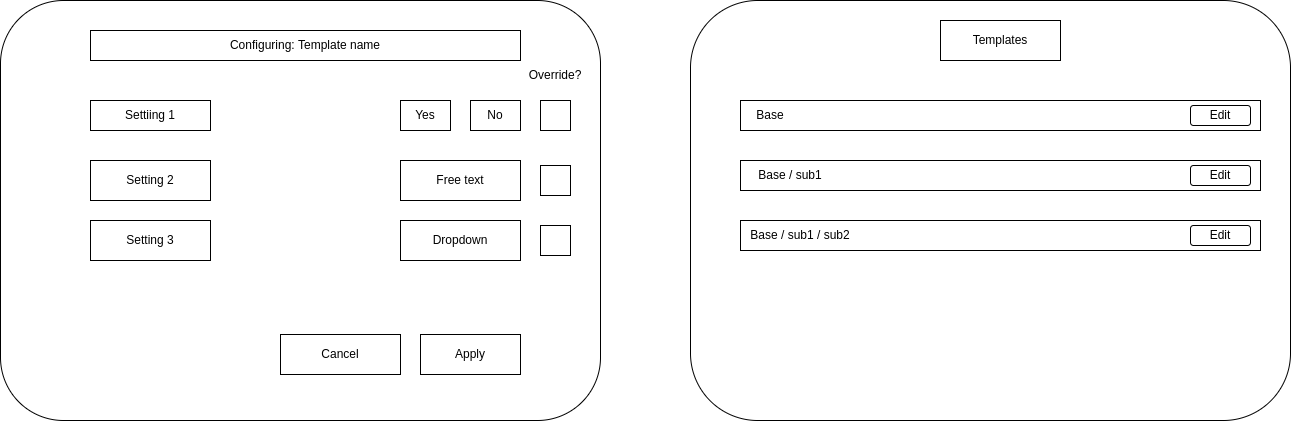
\includegraphics[scale=0.2]{wireframes}
	\caption{Template overview  wireframe}
	\label{fig:templatewireframe}
\end{figure}

\subsection{Design patterns}
TBD Integrate these where applicable instead of separately.

Design patterns are reusable solutions to commonly occurring software design problems. Design patterns are not ready made solutions that directly translate to machine readable code. Rather they are concepts that can be applied to solve a common problem in different situations. They may be seen as an intermediate between a programming paradigm (e.g. functional- or object-oriented programming) and
concrete algorithms. Design patterns can be divided in three categories, namely creational, behavioral and structural.

\subsubsection{Composite}
The composite pattern is a structural design pattern. With this design pattern objects can be grouped such that they are treated as a
single instance.

\subsubsection{Factory}
The factory method is a creational design pattern used for creating objects in a generic superclass that allows subclasses to change the
specific type of object that is created.

\chapter{Implementation}
\section{Development environment}
BauWatch has git repository templates for commonly used programming languages. These templates contain a standardized directory structure along with configuration
files for the Gitlab code pipelines. This makes it easy to start a project and immediately get started with a basic environment to run linters, documentation
generators and automatic tests.
%TODO Maybe add something about the tools used? These are gitlab (CI), GNU Make, golang tools, Docker. Might be useful to describe testing

\section{httprouter}
I use httprouter

%\section{Parameters not in parent}
%Parameters can optionally be overridden by the base templates children. This is implemented using a map.
%An issue arises when in child 2 param c is added. That param is not defined in child 1 or the base template.
%How can this param be set in the first place?
%Guard against this in the model and disallow adding parameters through the webpanel.
%Additionally the base template should be initialized from some presupplied default, be it yaml or constants.

\section{Template implementation}
Pics:
Struct, interactions between templates
Describe how template stacking works

\chapter{Testing}
Tests to be conducted:
Unit tests
System test

TBD

\chapter{Conclusion}
Unfortunately there was no time to implement all requirements.
Nevertheless there is enough evidence that supports the use of a generic system for configuring cameras.

\chapter{Recommendations}
If the configurable parameters grow in numbers it would be nice to separate them in different categories that can be folded.

Use git internal datastructure only

\chapter{Reflection}
At the start of my graduation period halfway through november, the winter season was approaching and COVID-19 infection rates were again going up.
As a result the country entered into another lockdown in an attempt to flatten the curve.
This unfortunately meant that working from home was again in effect.
This meant I was not able to meet a lot of people at the start of my internship and it took a while to get to know my colleagues.
While I was able to mostly work from the office in the first two weeks to get set up with the proper materials and to get to know my mentor I did not get to meet all of my team members until three months after starting.

While preparing the plan of approach some preliminary library research was done before fully digging into the research phase of the project.
During this period a previous thesis on creating an ,,ONVIF Plug-in" \cite{kesteloo_onvif_2016} was found.
This thesis was found to contain a lot of material that would have been produced within the original scope of the project.
Originally the project was aimed at creating software that could change camera settings through ONVIF to allow universal control.
After consulting with my mentor, graduation teacher and the graduation coordinator it was decided that the project could continue without delaying the project and going through the formalities of defining a new project if a adjusted proposal could be provided.
Unfortunately redefining the project meant that the plan of approach had to be adjusted with new research objectives and problem description and with some adjustments this was finally approved after the christmas break in the seventh week after the starting date.

It was recommended to me to implement the prototype in Go.
While I never programmed in Go and had to learn it from scratch I was interested in the language and since a lot of knowledge was present at BauWatch I did not want to dismiss it right away.
While my lack of experience did sometimes briefly impede my progress in order to grasp a new concept or to refactor some things because it did not work well in Go I did learn a lot about the language and got to appreciate it as a valuable tool to add to my repetoire.


covid
onvif
redefine project
plan of approach
new programming language Go
what went well
what went bad
lack of other interns
small company



% TODO: Remove this
\chapter{Research methodology} \label{methods}
Research methods are used according to the  In this chapter the methods that
will be used are described and their application will be handled in chapter \ref{activities}.
\section{Library}
Library research is done to explore what is already done and what guidelines and theories exist that could help you further your design. Since the advent of the internet library research is also called desk research.

\subsection{Available product analysis}
An available product analysis is the process of finding out if there are already existing solutions to the problem at hand.

\subsection{Best good and bad practices}
The best good and bad practices is a research method where work of others is investigated and a way is found to incorporate this in your own research.

\subsection{Literature study}
Literature study is used to gather information about a subject, determining what material to read in detail and summarising your findings.

\subsection{Design pattern research}
Design patterns are documented solutions to frequently encountered problems or challenges in software engineering; they incorporate good software engineering principles. Having good knowledge of these patterns can help improve the quality of designed software.

\section{Workshop}
Workshop research is done to explore opportunities. Prototyping, designing and co-creation activities are all ways to gain insights in what is possible and how things could work.

\subsection{Prototyping}
With this domain a prototype is built to show an idea to stakeholder and to evaluate if it is worth expanding upon.

\subsection{Requirements Prioritization}
This method can be used to gather requirements from stakeholders and will be used during the design phase of the project. Once the requirements have been determined a prioritization can be made so that they can be implemented based on priority.

\subsection{IT architecture sketching}
Come together around a whiteboard and draw the high-level architecture based upon discussion before and during the drawing process. Stay away from details, unless they are important for the overall design.

\subsection{Unit test}
Define one or more tests for each ‘atomic part’ of the code (e.g. a method or function). The unit should be tested in isolation.

\chapter{Activities} \label{activities}
The project is broken down into four phases consisting of the Definition, Analysis, Design and Implementation phase. Each phase is then further broken down into
research activities as described in section \ref{methods}.

\section{Project definition}
\subsection{Available product analysis}
During the definition phase of the project an available product analysis was done to evaluate relevant research done in the past that may be of relevance to this
project. During the analysis a thesis \cite{kesteloo_onvif_2016} was found that completed a lot of work that would have been done in the original scope of the project. After
this analysis the decision was made to move the scope of the project to prevent research from unnecessarily being repeated. With the new scope in mind the analysis was
conducted again and some solutions were found that could get and set settings from an ONVIF enabled camera but none were found that could create a generic configuration nor
were there generic solutions for cameras not implementing ONVIF.

\section{Analysis}
\subsection{Best good and bad practices}
The cameras that will be used implement multiple APIs, one more useful than the other. Before the design can be made it should be evaluated which API will be used and
how it works. The implementation of this API can have effect on certain parts of the design in regards to the chosen programming language, interface design and
implemented capabilities.

\subsection{Prototyping}
In order to gain a better understanding of the camera APIs some very simple proof of concepts can be built to gain experience with the API. This knowledge can then be applied during the design and implementation phases.

\section{Design}
\subsection{Design pattern research}
The prototype will include an interface between a generic configuration and the camera specific configurations. In order to make this interface future proof, design patterns should be researched so that the interface can be designed to be easily extended.

\subsection{IT architecture sketching}
During the design phase thought will be put into the architecture of the prototype. This will start with a sketch of the overall prototype and this will be refined into a functional and technical design.

\section{Implementation}
\subsection{Prototyping}
The functional and technical design will be implemented in the form of a prototype.

\subsection{Unit test}
To validate the operation of the prototype unit tests will be written to cover as many code paths as possible. Next to that an integration test will be done to validate
proper functioning of the prototype. The details of this test will be formalized at a later stage in a test plan.

\subsection{Code review}
In order to maintain the quality of the prototype, code reviews will be done on all pull requests that are to be included in the prototype. The review can be done by either the company mentor or another team member.

\chapter{Project management}
The project will be conducted using Scrum. Scrum is already used within the team at BTG and it was decided that the project would use the same process to easily communicate progress and impediments to the team.

Sprints will be set at two weeks and start after the sprint planning on Monday. Scrum activities will be done together with BTG's team when this makes sense. Story mapping, backlog refinement, sprint planning and the retrospective will not be integrated with the team as this would take time away from both the graduate student and the team, as their work is not directly related to each other nor would they have much to contribute to the other party during those sessions. The only persons in these meetings will be the graduate student and his mentor. Effectively this means that only the daily stand-up will be part of the team's stand-up so that the graduate student can share what he is working on and indicate if there are any impediments that the team can help resolve.

BTG has a separate environment for students in their systems. This way they can keep their own backlog without mixing in with work from other teams. Next to that they also have their own place to host documentation and keep their code. In case a student needs to have access to internal resources these can be made available on an as needed basis.

\chapter{Stakeholder analysis}
During the definition phase a couple of stakeholders were identified. They were identified based on the fact that the outcome of the project would have
some sort of effect on them. Thymo is conducting the project and has the biggest stake in it. Wouter and Silke are both software engineers within the
back-end team and after the project is finished might have to work with the resulting project. Silke in particular has indicated that he would be helped
by the outcome as he currently has to spend a lot of time of batching API calls through a script if a larger amount of cameras need to be configured.
Alex is a Product Manager within BauWatch that had some ideas about the project objective.

\begin{table}[h]
    \centering
    \caption{Stakeholders}
    \label{tab:stakeholders}
    \begin{tabular}{ | m{10em} | m{10em} | }
    \hline
    \textbf{Stakeholder} & \textbf{Type} \\
    \hline
    Thymo van Beers & Key figure \\
    \hline
    Wouter Horlings & Influencer
    \\ \hline
    Silke Hofstra & Influencer
    \\ \hline
    Alex van der Leij & Onlooker
    \\ \hline
    \end{tabular}
\end{table}
 
 %%%%%%%% Plan of Approach ends here!!!! %%%%%%
 %%%%%%%%%%%%%%%%%%%%%%%%%%%%%%%%%%%%%%%%%%%%%%%

% TODO Replace with bibtex in template
%\begin{thebibliography}{2}
%    \bibitem{tim_k_onvif}
%        ``ONVIF Plug-in", \textit{Tim Kesteloo}, [online]. Available: \url{https://hbo-kennisbank.nl/details/sharekit_hh:oai:surfsharekit.nl:15d206a2-dc4e-4dbd-9719-339793255ddd}. [Accessed: 01-12-2021]
%    \bibitem{dot_framework}
%        ``The DOT-Framework", \textit{HBO-i}, [online]. Available: \url{https://ictresearchmethods.nl/The_DOT_Framework}. [Accessed: 01-12-2021]
%    \bibitem{ti_wmc}
%        ``Twente Institute for Wireless and Mobile Communications", \textit{SALUS}, [online]. Available:
%        \url{https://www.sec-salus.eu/consortium/ti-wmc/}. [Accessed: 20-01-2022]
%	\bibitem{what_is_foreman}
%		``Foreman :: Introduction", \textit{Foreman authors}, [online]. Available:
%		\url{https://www.theforeman.org/introduction.html}. [Accessed: 16-02-2022]
%	\bibitem{foreman_hostgroups}
%		``Managing Hosts", \textit{Foreman authors}, [online]. Available:
%		\url{https://docs.theforeman.org/3.1/Managing_Hosts/index-foreman-el.html}. [Accessed: 16-02-2022]
%    % \bibitem{moscow}
%    % ``MoSCoW Analysis (6.1.5.2)". A Guide to the Business Analysis Body of Knowledge (2 ed.).
%    % International Institute of Business Analysis. 2009. ISBN 978-0-9811292-1-1
%\end{thebibliography}

\printbibliography

\end{document}
